\item \textbf{{[}ALVL/9597/2016/P2/Q1{]} }

Many elderly people spend later life in a nursing home. The Ministry
of Health (MOH) requires each nursing home to keep detailed care records
for each resident. Care staff make daily entries in the care records
about all aspects of resident care. These care records are currently
paper-based documents. There is no common format for the documents
that different nursing homes use. 

Care staff do not have computer access to medical records that each
resident\textquoteleft s doctor holds. Nurses at a nursing home need
to keep their own medical records and to consult with residents\textquoteleft{}
doctors.

The MOH is planning an initiative to computerise all care records
and would like all nursing homes to use a common design for care records.

The MOH will send a project proposal which is to be circulated to
all nursing homes. This is to find out which homes would consider
taking part in a pilot project. The MOH's aim is to introduce a pilot
system into a single nursing home.

The MOH needs to find a software house to design and implement the
computerised care record system. It will send the project proposal
to software houses.

At a later date, all nursing homes will use the new computer system.
\begin{enumerate}
\item {} 
\begin{enumerate}
\item State \textbf{four} topics you would expect to find in this project
proposal.\hfill{} {[}4{]}
\item Describe the purpose of this project proposal. \hfill{}{[}2{]}
\end{enumerate}
Following production of the project proposal. the initial activities
with their expected times are as follows:
\begin{center}
\begin{tabular}{|c|>{\raggedright}p{0.5\columnwidth}|c|}
\hline 
\textbf{Label} & \texttt{\textbf{\hspace{0.01\columnwidth}}}\textbf{Activity } & \textbf{Time (weeks)}\tabularnewline
\hline 
A & Send the project proposal document to all nursing homes. & 5\tabularnewline
\hline 
B & Circulate the project proposal document to a number of software houses. & 6\tabularnewline
\hline 
C & Review the feedback. Note which nursing homes and software houses
have expressed interest.  & 2\tabularnewline
\hline 
D & identify doctors who look after residents in homes that have expressed
interest. Hold a presentation meeting to explain the proposed project
to these doctors. & 5\tabularnewline
\hline 
E & Presentation event for the chosen nursing home. & 2\tabularnewline
\hline 
\end{tabular}
\par\end{center}

\end{enumerate}
The Program Evaluation and Review Technique (PERT) chart for these
initial activities is shown below. 
\begin{center}
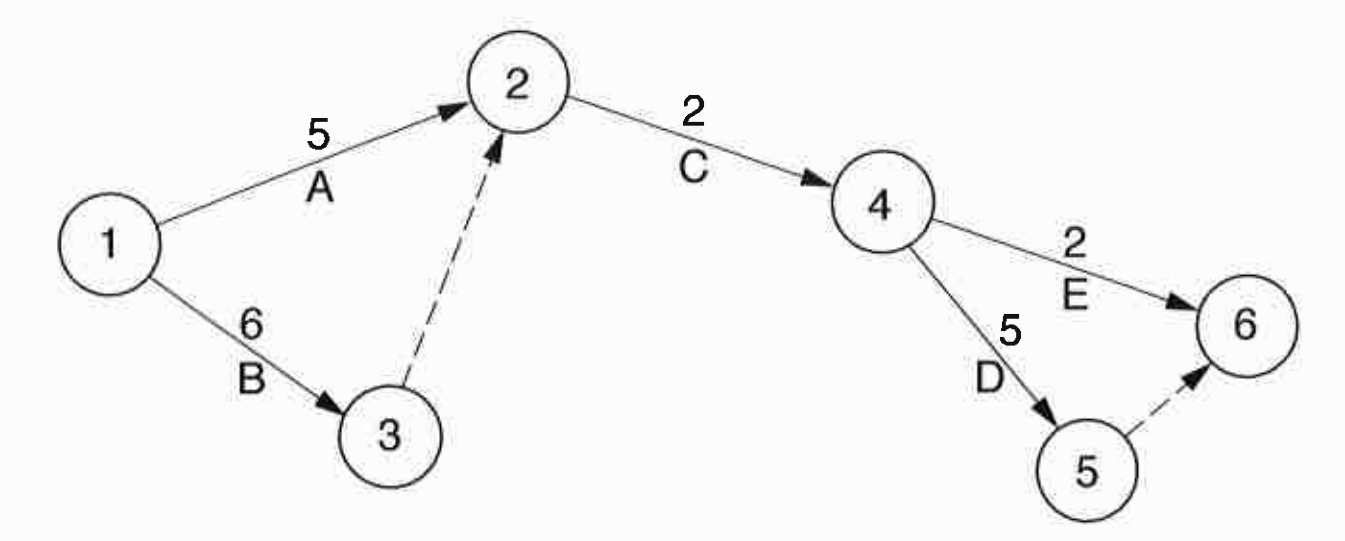
\includegraphics[width=0.5\paperwidth]{C:/Users/Admin/Desktop/Github/question_bank/static/img/9597-ALVL-2016-P2-Q1-1}
\par\end{center}
\begin{enumerate}
\item[(b)] {}
\begin{enumerate}
\item State the critical path for the initial activities. \hfill{}{[}1{]}
\item Calculate the minimum time these initial activities will take.\hfill{}
{[}1{]}
\end{enumerate}
\item[(c)] In activity E, the MOH presented more details about the project to
the manager and care staff of the chosen nursing home. The manager
and care staff raised a number of points about both social and ethical
issues associated with the project. 

Describe \textbf{three} points that could have been raised.\hfill{}
{[}6{]}
\end{enumerate}
Following activity E, the MOH decided the software house to which
it would award the contract. 

Following the initial project proposal. activities which make up the
system development cycle are shown below:
\begin{center}
\begin{tabular}{|c|>{\raggedright}p{0.5\columnwidth}|c|}
\hline 
\textbf{Label} & \texttt{\textbf{\hspace{0.01\columnwidth}}}\textbf{Activity} & \textbf{Time (weeks)}\tabularnewline
\hline 
F & Analysis & 12\tabularnewline
\hline 
G & Design & 15\tabularnewline
\hline 
H & Data entry of current care record data & 4\tabularnewline
\hline 
I & Initial testing & 10\tabularnewline
\hline 
J & Program development  & 14\tabularnewline
\hline 
K & Install new hardware in nursing home  & 3\tabularnewline
\hline 
L & Alpha testing & 2\tabularnewline
\hline 
M & Beta testing & 1\tabularnewline
\hline 
N & Implementation & 3\tabularnewline
\hline 
\end{tabular}
\par\end{center}

\begin{center}
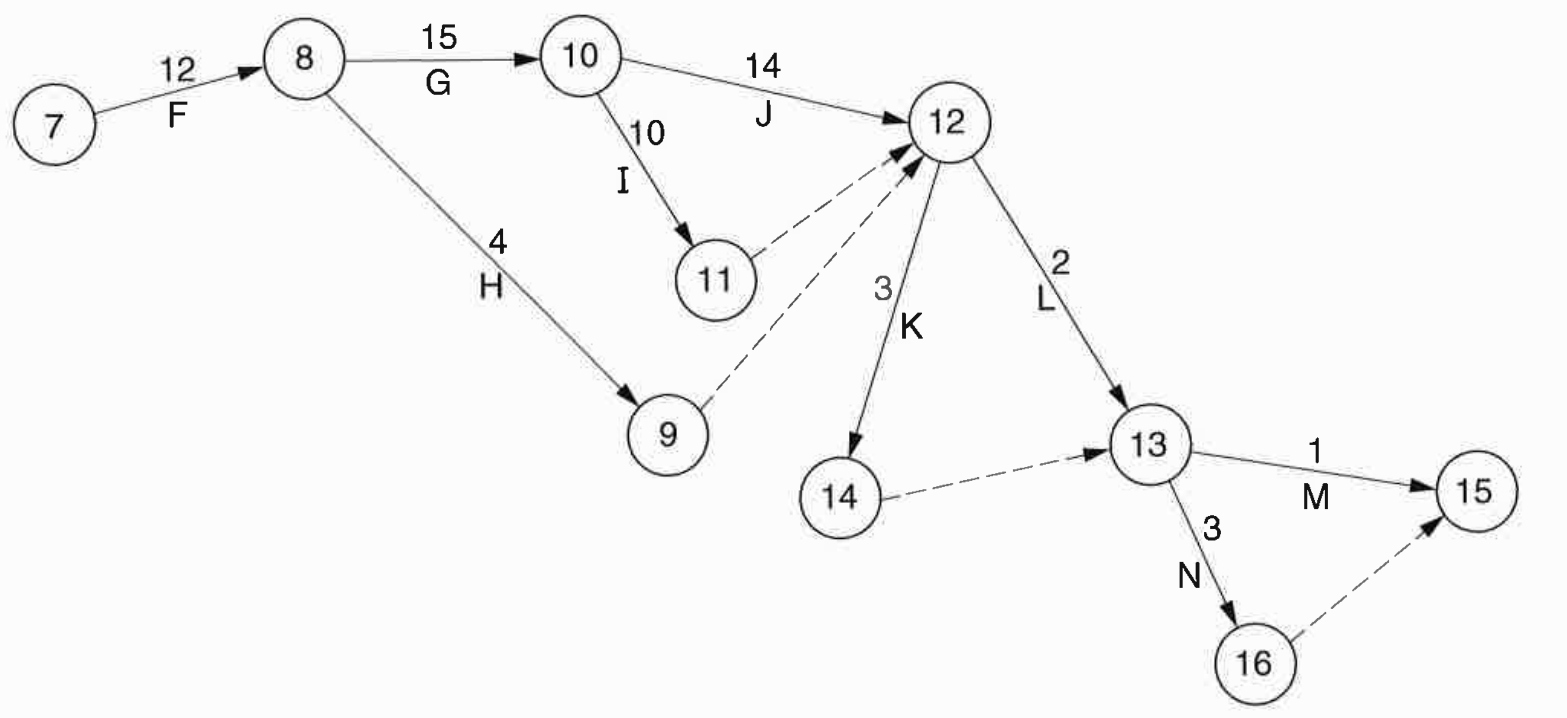
\includegraphics[width=0.5\paperwidth]{C:/Users/Admin/Desktop/Github/question_bank/static/img/9597-ALVL-2016-P2-Q1-2}
\par\end{center}
\begin{enumerate}
\item[(d)] The system development cycle starts at node (time point) 7.
\begin{enumerate}
\item The PERT chart shows four activities with dashed lines. Explain the
significance of the dashed lines.\hfill{} {[}1{]}
\item Explain the meanings of a dependent stage and concurrent stages in
a PERT chart. Give an example of each for this project. \hfill{}{[}4{]}
\item The table describes activity I as \textquoteleft initial testing'.
One category of initial testing is white-box testing.

Name and describe two other categories of initial testing. \hfill{}{[}4{]}
\item The PERT chart indicates that some testing can commence almost as
soon as program development does. Describe the type of program development
that would allow for this.\hfill{} {[}2{]}
\end{enumerate}
\item[(e)] An analyst from the software house carried out the analysis for the
project. 

Describe \textbf{three} examples of people whom the analyst consulted.
For each example. state: 
\begin{itemize}
\item the fact finding technique used 
\item the nature of the information that the analyst obtained. 
\end{itemize}
Each fact finding technique should be different.\hfill{} {[}6{]}
\item[(f)]  When the analysis stage was completed. the following decisions were
taken: 
\begin{itemize}
\item Each nursing home will store and manage its own care records data. 
\item Each nursing home will be provided with a local area network (LAN). 
\item The care record system on each LAN will use a client-server model
with a web interface for client computers. 
\end{itemize}
\begin{enumerate}
\item Explain the meaning of the term client-server model. \hfill{}{[}3{]}
\item State the \textbf{two} items of software that the LAN will use to
implement this client-server design. \hfill{}{[}2{]}
\end{enumerate}
\end{enumerate}
During the presentation event to doctors (part of activity D). the
doctors gave feedback. They said that they would like to have access
to the new computerised care records from their own offices. 
\begin{enumerate}
\item[(g)] A second phase of the project is to allow each nursing home access
to the medical data stored by doctors. This will involve connecting
the LAN for each nursing home to a number of doctors' surgery LANs. 
\begin{enumerate}
\item (l) State \textbf{two} methods for ensuring the security of access
to the care record network application. \hfill{}{[}2{]}
\item (ll) Give \textbf{two} methods for protecting the security of the
LAN. \hfill{}{[}2{]}
\end{enumerate}
\end{enumerate}